\documentclass[aspectratio=169,hyperref={pdfpagelabels=false}]{beamer}
\input{preamble.tex}

\subtitle{\normalsize{Industrial IoT for Digitization of Electronis Assets}}
\title{Model Predictive Control and Imitation Learning}

\setdepartment{DTU Wind and Energy System}
\setcolor{blue}

\begin{document}
\inserttitlepage

%B SLIDE 0
\begin{frame}{Agenda}
    \begin{itemize}
        \item Introduction
        \item Overview of MPC
        \item System Model
        \item Objective Function
        \item Constraints and Optimization
        \item Learning Agent
        \item Conclusion
    \end{itemize}
\end{frame}

\begin{frame}
  \frametitle{Overview of MPC}
  \begin{itemize}
      \item Model Predictive Control (MPC) is an advanced method of process control that predicts the future behavior of a system.
      \item MPC uses a mathematical model to make predictions and optimize control actions.
      \item It handles multi-variable control problems with constraints effectively.
  \end{itemize}
  \end{frame}
  
  \begin{frame}
  \frametitle{System Model}
  \begin{itemize}
      \item The system is typically represented by a state-space model:
      \[ x_{k+1} = Ax_k + Bu_k + w_k \]
      \[ y_k = Cx_k + v_k \]
      \item \( x_k \): state vector, \( u_k \): control input, \( y_k \): output.
      \item \( A, B, C \): system matrices, \( w_k, v_k \): process and measurement noise.
  \end{itemize}
  \end{frame}
  
    
\begin{frame} \frametitle{MPC: The Objective Function}
  Objective function to be minimized over a prediction horizon \( T \):
  \begin{equation*}
    \begin{aligned}
    \min_{u, x, y} \quad & \sum_{k=0}^{T} \|y_{k} - r_{k}\|^2_Q + \|u_{k}\|^2_R \\
    \textrm{s.t.} \quad & x_{k+1} = Ax_k + Bu_k, \quad \forall \: \textbf{k} \: \in \{\textbf{1}, \dots, \textbf{T}\}\\
      &y_{k} = Cx_k + D u_k, \quad \hspace{0.8em} \forall \: \textbf{k} \: \in \{\textbf{1}, \dots, \textbf{T}\}\\
    \end{aligned}
  \end{equation*}
  \begin{itemize}
      \item \( y_{k} \): predicted output, \( r_{k} \): reference output, \( u_{k} \): predicted control input.
      \item \( Q, R \): weighting matrices for tracking error and control effort.
  \end{itemize}
    
    \let\thefootnote\relax\footnotetext{\tiny{\textcolor{blue}{\url{https://www.youtube.com/watch?v=sKQqAeJMzBk&t=1838s&ab_channel=ControlMeetsLearning}}}}
\end{frame}




  \begin{frame}
  \frametitle{Constraints and Optimization}
  \begin{itemize}
      \item MPC can handle various constraints like input, state, and output constraints.
      \item Optimization problem solved at each step to find the best control sequence.
      \item Receding horizon principle: Only the first control action is implemented and then the horizon is updated.
  \end{itemize}
  \let\thefootnote\relax\footnotetext{\tiny{\textcolor{blue}{\url{https://www.youtube.com/watch?v=YwodGM2eoy4&ab_channel=SteveBrunton}}}}
  \end{frame}

\begin{frame}{Example}
  Let's consider a simple example, where the goal is to control the temperature of a room.
  \begin{itemize}
      \item The temperature of the room is the output variable.
      \item The control input is the power of the heater.
      \item The reference output is the desired temperature.
  \end{itemize}
  And that the system is described by the following equation:
  \begin{align*}
    T_{new} = T_{current} + P_{[\%]\: heater}\times 0.1 \times \Delta  T
  \end{align*}\pause
  \begin{block}{}
    \textbf{Question:} How can we control the temperature of the room?
  \end{block}
  \end{frame}

  \begin{frame}{Example}
    \begin{align*}
      T_{new} = T_{current} + P_{[\%]\: heater}\times 0.1 \times \Delta  T
    \end{align*}

    Given:
    \begin{itemize}
        \item $T_{current} = 20 \: ^{\circ} \text{C}$
        \item $T_{desired} = 22 \: ^{\circ} \text{C}$
        \item $T_{output} = 18 \: ^{\circ} \text{C}$
        \item $\Delta T = T_{output} - T_{current} =  -2 \: ^{\circ} \text{C}$
    \end{itemize}
    \begin{align*}
    \textbf{HOUR 1:} \quad T_{new} = 20 ^{\circ} \text{C} + \textbf{U}\% \times 0.1 \frac{^{\circ} \text{C}}{{\%}} - 2 \longrightarrow \textbf{U} = 40 \% \\
    \end{align*}
So we need to set the heater to 40\% for the first hour. Once the first hour is over, we can update the system model and repeat the process.
\end{frame}
 
\begin{frame}{\normalsize{A MPC controller to increase the Energy Efficiency of a Wastewater Station}}
  \begin{figure}
    \centering
    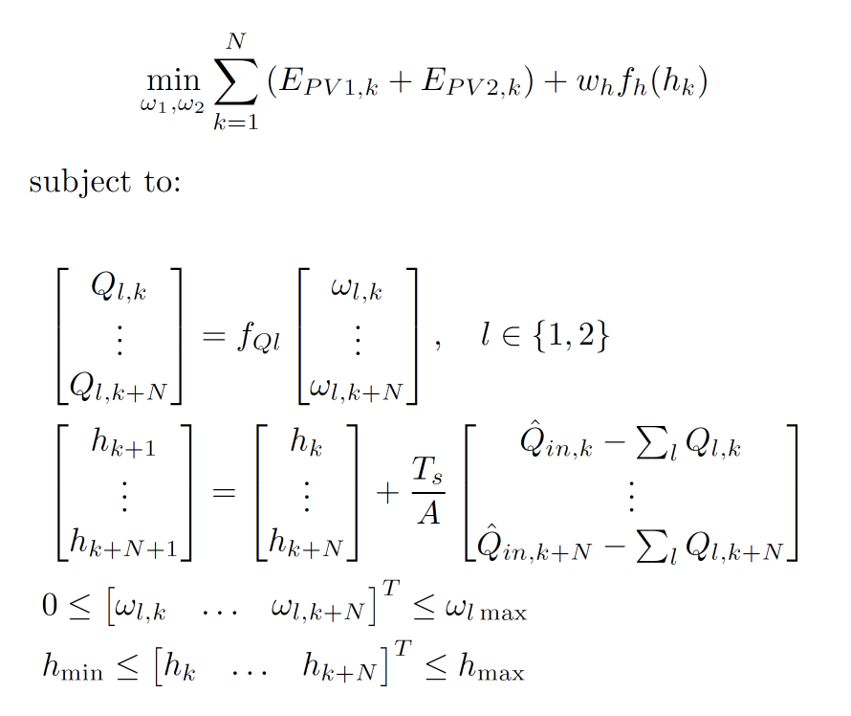
\includegraphics[width=0.60\textwidth]{img/mpc_formulation.png}
    \label{fig:image}
  \end{figure}
\end{frame}

  \begin{frame}
  \frametitle{Summary:}
  \begin{itemize}
      \item MPC is a powerful control strategy for systems with predictive models.
      \item Its ability to anticipate and optimize future behavior makes it applicable in various fields.
      \item The optimization formulation is key to its effectiveness.
  \end{itemize}
  \end{frame}

  \begin{frame}
    \frametitle{Challenges in MPC Deployment}
    \begin{itemize}
        \item Solving optimization problems online is computationally demanding.
        \item High-dimensional systems pose a challenge due to the complexity and required computational resources.
        \item Strict latency requirements and limited computational or energy resources can impede the deployment of MPC.
    \end{itemize}
    \let\thefootnote\relax\footnotetext{\tiny{Ahn, Kwangjun, et al. "Model Predictive Control via On-Policy Imitation Learning." Learning for Dynamics and Control Conference. PMLR, 2023.}}
    \end{frame}


    \begin{frame}
      \frametitle{Interactive Data Collection Scheme}
      \begin{itemize}
          \item A scheme is proposed to interactively collect data from a system in feedback with an MPC controller.
          \item The goal is to learn an explicit controller that directly maps states to inputs.
          \item This methodology aligns with imitation learning approaches in the reinforcement learning domain.
      \end{itemize}
      \vfill
      \let\thefootnote\relax\footnotetext{\tiny{Ahn, Kwangjun, et al. "Model Predictive Control via On-Policy Imitation Learning." Learning for Dynamics and Control Conference. PMLR, 2023.}}
    \end{frame}
      

      \begin{frame}
        \frametitle{Imitation Learning and MPC}
        \begin{itemize}
            \item Imitation learning involves learning an explicit controller that maps states to inputs.
            \item It is suitable for MPC as it can query the MPC for the next input at any state by solving the optimization problem.
            \item This process aligns with explicit MPC, which pre-computes solutions to optimization problems for runtime efficiency.
        \end{itemize}
      \let\thefootnote\relax\footnotetext{\tiny{Ahn, Kwangjun, et al. "Model Predictive Control via On-Policy Imitation Learning." Learning for Dynamics and Control Conference. PMLR, 2023.}}
        \end{frame}

        \begin{frame}
          \frametitle{Learning Controllers with High Fidelity to MPC}
          \begin{itemize}
              \item The goal is to learn a map from states to inputs that encapsulates the strategy of an MPC controller.
              \item Unlike methods that collect data pre-learning, our approach interacts with the system dynamics to avoid distribution shift.
              \item This interaction prevents sub-optimal performance and error compounding, which are common in non-interactive imitation learning.
              \item Our approach aims for a learned controller that matches MPC performance with high probability.
          \end{itemize}
      \let\thefootnote\relax\footnotetext{\tiny{Ahn, Kwangjun, et al. "Model Predictive Control via On-Policy Imitation Learning." Learning for Dynamics and Control Conference. PMLR, 2023.}}
          \end{frame}
          
          \begin{frame}
            \frametitle{Imitation Learning from an Expert}
            \begin{block}{}
              \textbf{Imitation learning} aims to learn the optimal controller ${\hat{\pi}}$ by minimizing the loss function $L(\pi)$ with respect to the MPC controller. 
              \begin{align*}
                \min_{W,b} J(W, b) = \frac{1}{N} \sum_{i=1}^{N} (\hat{\omega}_{i}^2 -\omega_{i}^{opt}) + \lambda \sum_{k} \sum_{j} w_{k,j}^2 \quad l \in \{1, 2\}
              \end{align*}
            \end{block}
            \let\thefootnote\relax\footnotetext{\tiny{Quattrociocchi, Alessandro, et al. "Energy Efficiency Optimization of a Wastewater Pumping Station Through IoT and AI: A Real-World Application of Digital Twins." IECON 2023-49th Annual Conference of the IEEE Industrial Electronics Society. IEEE, 2023.}}
            \end{frame}

          \begin{frame}{All the Loss function seen so far...}
            \begin{block}{Paramaters Estimation in ARX Model}
              \begin{align*}
                \mathcal{L}(\theta, Z^N) = \sum_{k=0}^{N-1}(y(t)-\hat{y}(t|\theta))^2 = \sum_{k=0}^{N-1}(y(t)-\varphi'(t)\theta)^2 
              \end{align*}
            \end{block}
          \end{frame}

          \begin{frame}{All the Loss function seen so far...}
            \begin{block}{MPC Objective Function}
                \begin{align*}
                \min_{u, x, y} \quad & \sum_{k=0}^{T} \|y_{k} - r_{k}\|^2_Q + \|u_{k}\|^2_R
                \end{align*}
            \end{block}
          \end{frame}

          \begin{frame}{All the Loss function seen so far...}
            \begin{block}{Neural Network Loss Function}
              \begin{align*}
                \min_{W,b} J(W, b) = \frac{1}{N} \sum_{i=1}^{N} (\hat{\omega}_{i}^2 -\omega_{i}^{opt}) + \lambda \sum_{k} \sum_{j} w_{k,j}^2 \quad l \in \{1, 2\}
              \end{align*}
            \end{block}
          \end{frame}

          \begin{frame}{Some Resources: }
            \begin{itemize}
              \item \href{https://www.youtube.com/watch?v=0Ey02HT_1Ho&ab_channel=SteveBrunton}{\textcolor{blue}{\underline{Model Predictive Control in a Nutshell}}}
              \item \href{https://alexlenail.me/NN-SVG/}{\textcolor{blue}{\underline{Visualize and Draw the Structure of a Neural Network}}}
              \item \href{https://playground.tensorflow.org}{\textcolor{blue}{\underline{Visualize the Training of a Neural Network Online}}}
              \item \href{https://www.youtube.com/watch?v=L_4BPjLBF4E&ab_channel=AIWarehouse}{\textcolor{blue}{\underline{Reinforcement Learning Agent Simulation}}}
            \end{itemize}
          \end{frame}
\end{document}